%================================================================================
%       Safety Critical Systems Club - Data Safety Initiative Working Group
%================================================================================
%                       DDDD    SSSS  IIIII  W   W   GGGG
%                       D   D  S        I    W   W  G   
%                       D   D   SSS     I    W W W  G  GG
%                       D   D      S    I    WW WW  G   G
%                       DDDD   SSSS   IIIII  W   W   GGG
%================================================================================
%               Data Safety Guidance Document - LaTeX Source File
%================================================================================
%
% Description:
%   Worked Example section.
%
%================================================================================
\chapter{Worked Example (Informative)} \label{bkm:workedexample}

\dsiwgSectionQuote{There is a forest of data and we need to create a path through.}{Tom Adams}

\section{Purpose}
This section provides a worked example of applying the \gls{dsg} to a hypothetical system in the healthcare sector. Although some aspects of the example have been simplified, it is intended to be sufficiently realistic to allow key features of the guidance to be illustrated.

\section{Establish Context}

\subsection{Background}
A manufacturer is building a new integrated health and social care system to support holistic care for community health services. The system will support clinical workflows for aspects such as referrals, tracking clinical encounters, appointment scheduling, outcome measures through to letter and report generation. The development will follow a typical development lifecycle\index{Lifecycle!System} as a series of phases: business modelling, requirements, analysis and design, implementation, test, and deployment. 

\begin{figure}[H]
  \centering
  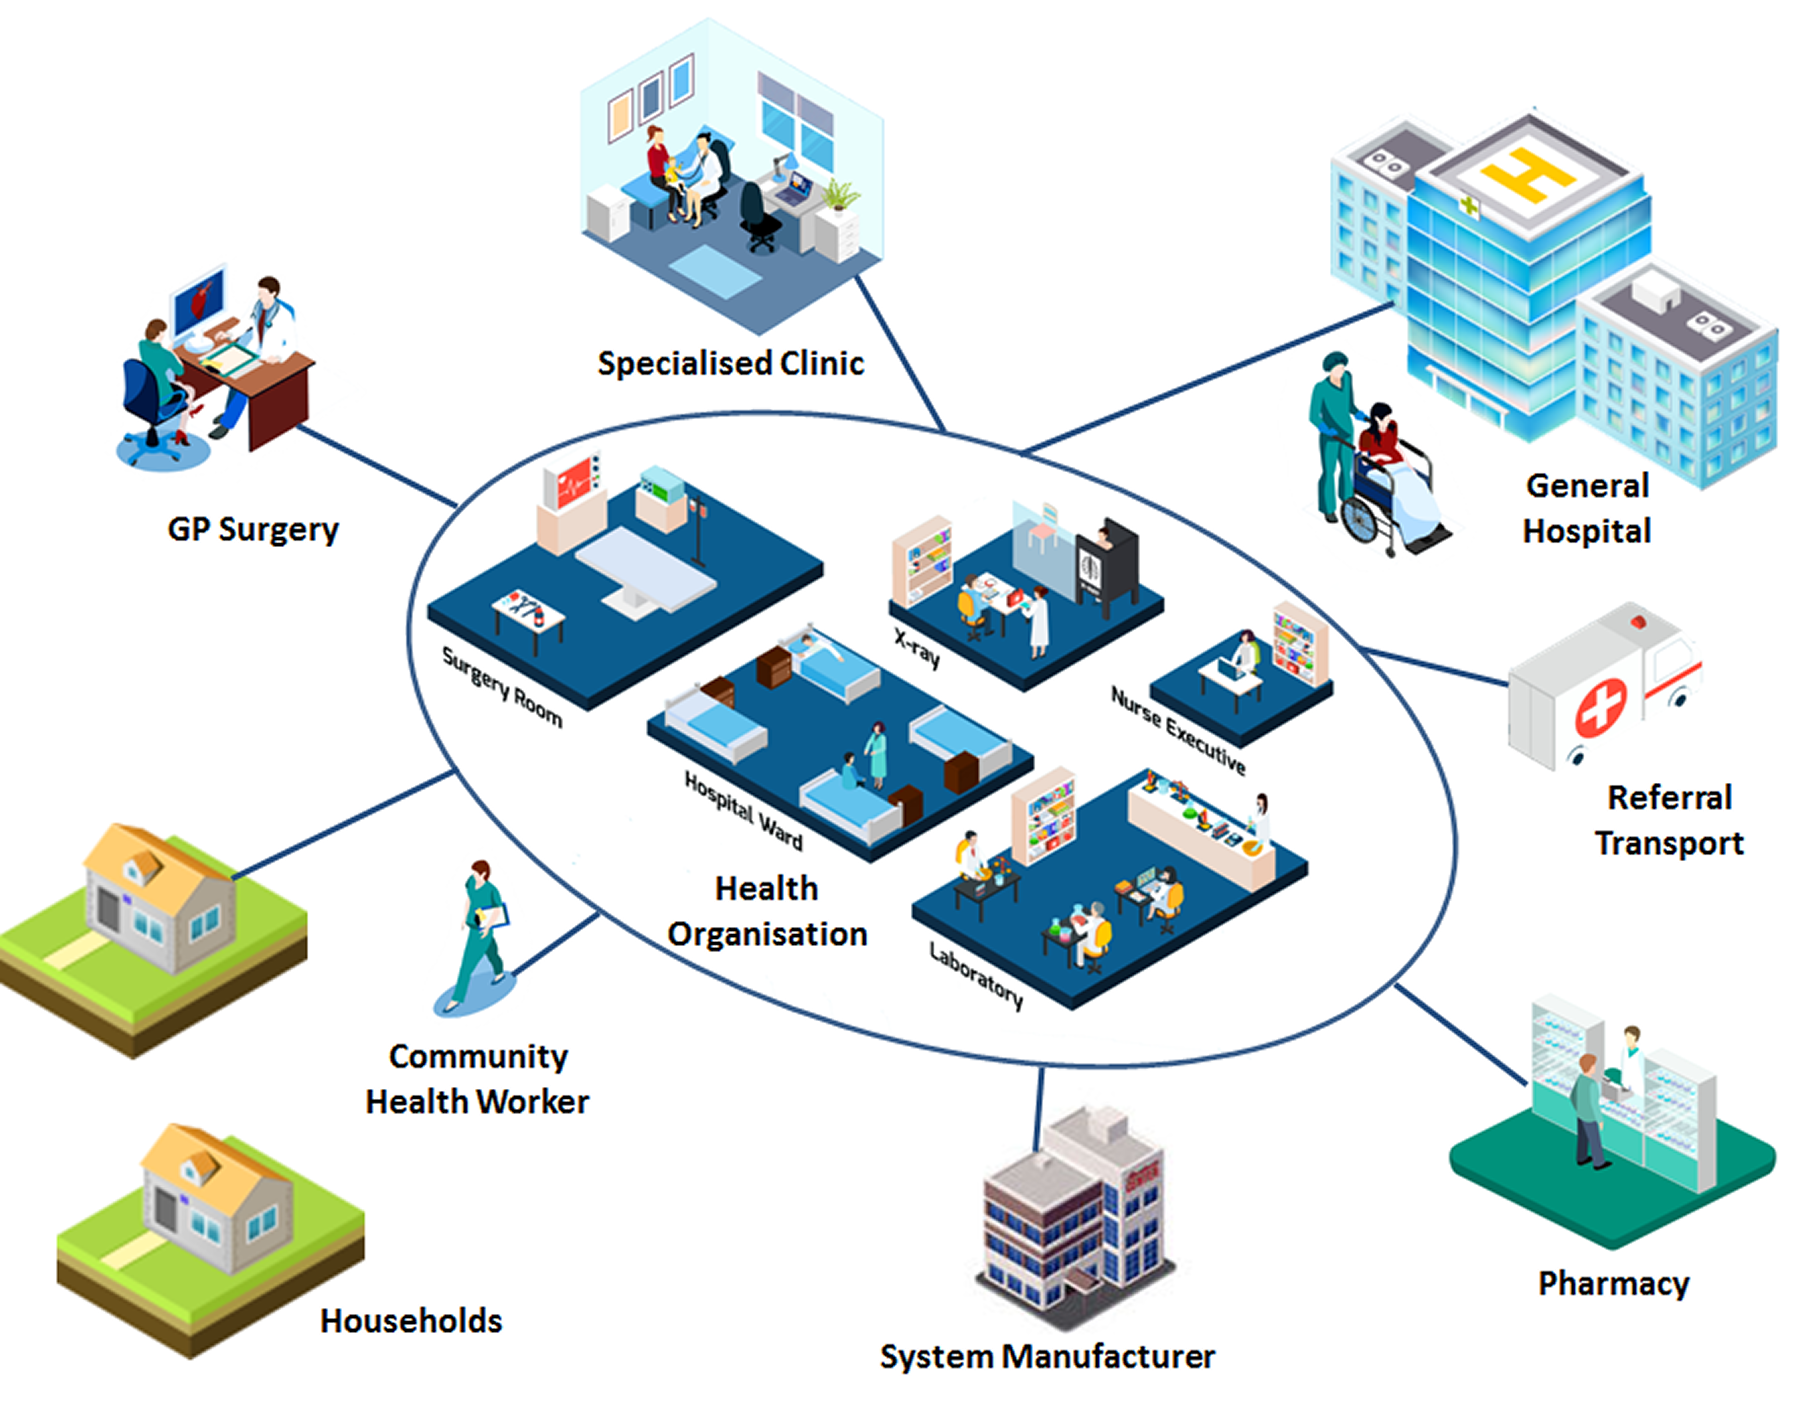
\includegraphics[width=0.9\textwidth]{images/medicalscenario}
  \label{fig:medicalscenario}
\end{figure}

\clearpage
The system is being targeted to meet the requirements of a health organization that is procuring a solution to help their clinicians maintain a high level of quality of care in the face of increasing volumes of patients and pressure to reduce staff costs.

Fundamental to fulfilling these requirements is establishing the context within which data is used in system development, enhancement, introduction, integration or operation. This should establish the risk appetite: essentially, how much effort is to be devoted to making data risks as low as practicable. In turn, this will inform the nature and scope of assessments that are to be conducted during system development and its introduction into operational service. To meet the `establish context' objectives set out in the guidance the following activities are recommended:

\begin{itemize}
	\item describe the organizational context;
	\item describe the system context;
	\item plan the assessment; and
	\item identify \glspl{data artefact}.
\end{itemize}

%
%Put text and image next to each other on the page.
%There are a number of ways of doing this, none of which are that nice or work that well.
%We could use the 'wrapfig' package but it's prone to errors in placement and running outside of page boundaries
%
\begin{minipage}[t][2cm]{0.73\textwidth}
  The manufacturer decides to use an \gls{odr} assessment form to understand in broad terms the level of risk it will have to manage in developing and supporting this system. This will allow the manufacturer to describe the organizational context and describe the system context.
\end{minipage}
\begin{minipage}[c][1cm]{0.25\textwidth}
	\vspace{1cm}
  \centering
    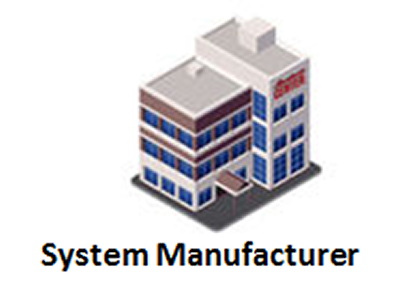
\includegraphics[width=\textwidth]{images/manufacturer}
\end{minipage}

\subsection{\Glsfmtshort{odr} Assessment}
The manufacturer considered each of the questions within the \gls{odr} form from\autoref{bkm:assessment} of this document.
The questions in the \gls{odr} and the manufacturer's assessments were:

% Miktex allocates table numbers to starred longtable* commands - don't know if this is specific to Miktex, a bug, or a change.
% But I've changed the unnumbered tables to description environments to remove the problem.

\addtocounter{table}{-1} % Kludge because longtable* is wrongly incrementing the table counter
\begin{longtable*}[H]
	{|L{\dsiwgColumnWidth{0.06}}|L{\dsiwgColumnWidth{0.94}}|}
	\hline
	Q1: & How severe could an accident be that is related to the data? Could it be caused directly by the data?\\
	\hline
\end{longtable*}

Failings in the system could give rise to non-optimal \index{Treatment!Medical}treatment plans for a patient that might delay detection of a more serious condition or prolong the recovery for a known condition. The system could not directly cause an accident, however, and there are other people and systems in play involved in checking data. On balance, this question is assessed as \dsiwgTextBF{1c}; Score \dsiwgTextBF{4}.

\addtocounter{table}{-1} % Kludge because longtable* is wrongly incrementing the table counter
\begin{longtable*}[H]
	{|L{\dsiwgColumnWidth{0.06}}|L{\dsiwgColumnWidth{0.94}}|}
	\hline
	Q2: & What would be the impact on the organization, client or public if an accident occurred related to the data?\\
	\hline
\end{longtable*}

Unfortunately, accidents in the health domain are relatively frequent. There are many injuries and deaths attributed to medical errors, but these are largely tolerated by the public and grievances are usually settled  by financial settlements through the courts. The manufacturer believes their contractual arrangements mean that the health organization would be liable for any claims even if they were attributed to an error in the manufacturer's system's handling of data. On balance, this question is assessed as \dsiwgTextBF{2b}; Score \dsiwgTextBF{2}.

\addtocounter{table}{-1} % Kludge because longtable* is wrongly incrementing the table counter
\begin{longtable*}[H]
	{|L{\dsiwgColumnWidth{0.06}}|L{\dsiwgColumnWidth{0.94}}|}
	\hline
	Q3: & How much responsibility does this organization have for data safety?\\
	\hline
\end{longtable*}

The manufacturer is responsible for building the system in compliance with
DCB0129 \cite{citation:dcb0129clinical}
and so is responsible for executing the associated safety management system to manage risk. The manufacturer, however, plans to sell the product with a condition of use that places end responsibility for patient safety on the client. On balance, this question is assessed as \dsiwgTextBF{3b}; Score \dsiwgTextBF{2}.

\addtocounter{table}{-1} % Kludge because longtable* is wrongly incrementing the table counter
\begin{longtable*}[H]
	{|L{\dsiwgColumnWidth{0.06}}|L{\dsiwgColumnWidth{0.94}}|}
	\hline
	Q4: & What legal and regulatory environment will this work be subject to?\\
	\hline
\end{longtable*}

The work will be contracted under UK law and subject to the \gls{dcb}
standards for health IT Systems. However, there is no regulator currently empowered to intervene in the delivery of healthcare systems, so the standards are not currently enforced through law. Instead, the health organization will make compliance with the standards a contractual requirement. On balance, this question is assessed as \dsiwgTextBF{4c}; Score \dsiwgTextBF{4}.

\addtocounter{table}{-1} % Kludge because longtable* is wrongly incrementing the table counter
\begin{longtable*}[H]
	{|L{\dsiwgColumnWidth{0.06}}|L{\dsiwgColumnWidth{0.94}}|}
	\hline
	Q5: & How mature is this organization regarding data safety?\\
	\hline
\end{longtable*}

The manufacturer has a good understanding of data as a source of safety risk. Many of their systems are data intensive to support clinical decision making. There is good support and funding for the identification and treatment\index{Treatment!Risk} of data-related risks. On balance, this question is assessed as \dsiwgTextBF{5b}; Score \dsiwgTextBF{2}.

\addtocounter{table}{-1} % Kludge because longtable* is wrongly incrementing the table counter
\begin{longtable*}[H]
	{|L{\dsiwgColumnWidth{0.06}}|L{\dsiwgColumnWidth{0.94}}|}
	\hline
	Q6: & How widely used is the data and who by?\\
	\hline
\end{longtable*}

The data will be used in multiple clinical settings and by many clinicians and other support staff. There are several data supply chains and public web access to data. On balance, this question is assessed as \dsiwgTextBF{6c}; Score \dsiwgTextBF{4}.

\addtocounter{table}{-1} % Kludge because longtable* is wrongly incrementing the table counter
\begin{longtable*}[H]
	{|L{\dsiwgColumnWidth{0.06}}|L{\dsiwgColumnWidth{0.94}}|}
	\hline
	Q7: & What is the scale, sophistication and complexity of the data and its manipulation?\\
	\hline
\end{longtable*}

The data is complex and although transmitted through industry standard data structures these require knowledge of the associated abstract clinical data model. Some data manipulation is required to map between different encodings of data held in the various heterogeneous systems. Some legacy systems transfer data in unstructured format. On balance, this question is assessed as \dsiwgTextBF{7c}; Score \dsiwgTextBF{4}.

\addtocounter{table}{-1} % Kludge because longtable* is wrongly incrementing the table counter
\begin{longtable*}[H]
	{|L{\dsiwgColumnWidth{0.06}}|L{\dsiwgColumnWidth{0.94}}|}
	\hline
	Q8: & How well defined and understood are the boundaries and interfaces for this data scenario?\\
	\hline
\end{longtable*}
The boundaries of the supply are well understood and although the interfaces are complex and mixed formats, these will be defined and agreed formally through \glspl{icd}. Most of the integrating systems are established \gls{cots} based systems, but some of the legacy systems still need to be investigated and working assumptions have been
made by the manufacturer. On balance, this question is assessed as \dsiwgTextBF{8c}; Score \dsiwgTextBF{4}.

The final score is \dsiwgTextBF{26}, which corresponds to \dsiwgTextBF{ODR2}. The manufacturer therefore concludes that there is low to medium risk that loss of \index{Property!Data}properties of data in the system can contribute to or give rise to harm. The manufacturer has an internal policy for engagements based on the \gls{odr} level that dictates how the organization will plan the assessment. This policy dictates the amount of proportional effort the manufacturer needs to spend on safety data management and the level of rigour to be employed. In this case, the policy dictates, amongst other requirements, that a separate section covering safety data management is required in its clinical risk management plan.

Next, the manufacturer identifies \glspl{data artefact} that are potential sources of safety hazards. The manufacturer knows that the safety dependency of data is dictated by the context in which it is used so it also develops an understanding of when in its process lifecycle\index{Lifecycle!Process} the data will be used and relied upon. The manufacturer plans to build an early prototype to show to clients to help elicit requirements definition. To support this, the manufacturer plans to create a test \gls{dataset} that comprises a typical range of scenarios that the system will encounter. This form of data is identified as \gls{verification} data. The system also needs to be configured to support deploying health organizations' policies. This data is infrastructure data\index{Infrastructure Data} and, for the prototyping phase, the manufacturer plans to use largely default values.

In later phases, when the system functionality is specified and the system is being built, the manufacturer plans to create a test \gls{dataset} that will be key to demonstrating the correct functioning of the system and hence acceptance by the deploying health organization. This still involves the use of \gls{verification} data\index{Verification Data} and infrastructure data\index{Infrastructure Data} but there will be far greater dependency on these \glspl{dataset} than the prototyping case. The manufacturer therefore documents in the clinical risk management plan the planned use of each of the data categories\index{Category!Data} during the entire delivery lifecycle\index{Lifecycle!Delivery}.

\begin{minipage}[t]{0.73\textwidth}
	The procuring health organization will have a different perspective of the IT system that it will deploy into its organization. It will already have many integrated systems in live operation and as part of establishing the context for the system's deployment they will need to consider many different types of \glspl{dataset}:
\end{minipage}
\begin{minipage}[t]{0.25\textwidth}
  \centering\raisebox{\dimexpr \topskip-\height}{%
    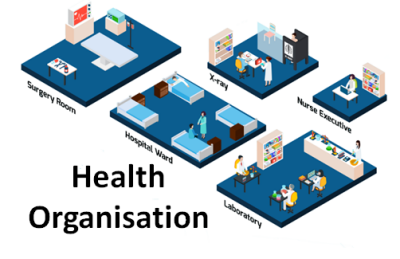
\includegraphics[width=\textwidth]{images/healthorganisation}}
\end{minipage}
	\begin{description}
		\item[Infrastructure data:]\index{Infrastructure Data} how the system will be configured in the specific environment;
		\item[\Glsfmttext{verification} data:]\index{Verification Data} the test \glspl{dataset} to be used to support certain deployments such as integration testing and training\index{Training!Personnel}; and
		\item[Dynamic data:]\index{Dynamic Data} the data entered or fed into the system and the data presented to the user, generated in the form of reports or data passed to other systems.
	\end{description}

The health organization decides to complete an \gls{odr} assessment
so it can describe the organizational context and describe the system context. The scoring is similar to the manufacturer with the following notable differences:

\addtocounter{table}{-1} % Kludge because longtable* is wrongly incrementing the table counter
\begin{longtable*}[H]
	{|L{\dsiwgColumnWidth{0.06}}|L{\dsiwgColumnWidth{0.94}}|}
	\hline
	Q2: & What would be the impact on the organization, client or public if an accident occurred related to the data?\\
	\hline
\end{longtable*}

The health organization would bear the brunt of any publicity and litigation in the event of an accident and so assesses this question as \dsiwgTextBF{2c}, Score \dsiwgTextBF{4}.

\addtocounter{table}{-1} % Kludge because longtable* is wrongly incrementing the table counter
\begin{longtable*}[H]
	{|L{\dsiwgColumnWidth{0.06}}|L{\dsiwgColumnWidth{0.94}}|}
	\hline
	Q3: & How much responsibility does this organization have for data safety?\\
	\hline
\end{longtable*}

The health organization is responsible for deploying systems in compliance with
DCB0160 \cite{citation:dcb0160clinical}
and is ultimately responsible for patient safety. The health organization assesses this as \dsiwgTextBF{3e}, Score \dsiwgTextBF{12}.

\addtocounter{table}{-1} % Kludge because longtable* is wrongly incrementing the table counter
\begin{longtable*}[H]
	{|L{\dsiwgColumnWidth{0.06}}|L{\dsiwgColumnWidth{0.94}}|}
	\hline
	Q5: & How mature is this organization regarding data safety?\\
	\hline
\end{longtable*}

The health organization has only recently acquired the expertise to apply
DCB0160
and is still developing its capability. Safety data management is new to the organization and it anticipates some resistance from senior management to the expenditure incurred in rolling out a DCB0160 compliant safety management system. This question is assessed as \dsiwgTextBF{5d}, Score \dsiwgTextBF{7}.

The resulting score for the health organization is \dsiwgTextBF{43}. This is \dsiwgTextBF{ODR3}: medium to high risk.
The health organization aims to plan the assessment through a clinical risk management plan. This plan defines the organization and system context in more detail and lays out the planned activities for identifying, evaluating and treating data safety related risks.

As with the manufacturer, the health organization needs to identify \glspl{data artefact} that are potential sources of safety hazards and understand the context of their use in the procurement / deployment lifecycles of the health organization\index{Lifecycle}.
Post acceptance, the procuring health organization plans to run a series of user training\index{Training!Personnel} sessions for clinicians.
Once users are trained, the system will be integrated into live operations.
The health organization identifies the infrastructure\index{Infrastructure Data},
\gls{verification}\index{Verification Data} and dynamic\index{Dynamic Data} data categories to be used
during these phases.
The health organization also realises that the system will form part of a data supply chain, because a number of external organizations and departments within their own organization engage in the procurement and use of safety-related data.
For example, it will receive referral data from a number of other \gls{gp} systems, it will receive outcome measures from hospitals, and it will receive clinical data acquired from remote workers visiting patients in the community and from the patients themselves using the system's online portal.
The system also produces data for other external systems such as electronic prescriptions for pharmacies.

The health organization sees that by using the new system it will become a commissioning user, as it will require and be a consumer of data from a variety of sources: \gls{gp} systems, hospital systems, systems used by remote workers in the community, and the system's portal capturing data entered by the patients themselves. All of these act as data provisioners. Those health care professionals patients gathering patient data through physical inspections and measurement are the data acquirers.

The health organization defines in its clinical risk management plan the data supply chain relevant to the system including the roles and interfaces involved. This will therefore show where there are dependencies on dynamic data used and produced by the system.

Questions the health organization will need to address when establishing the context are:
\begin{itemize}
  \item have all the dependent interfaces been identified?
  \item have the roles of commissioning user / data provider / data acquirer been established and acknowledged?
  \item what service level agreements or contracts exist for the delivery of the data?
  \item what level of assurance do data providers / data acquirers provide for their data?
\end{itemize}

\section{Risk Identification}
\begin{minipage}[t]{0.73\textwidth}
  The manufacturer aims to carry out the following activities to meet the guidance objectives for the risk Identification phase:
  \begin{itemize}
    \item review the general, historical perspective;
    \item conduct a top-down approach;
    \item conduct a bottom-up approach; and
    \item update planning documents.
  \end{itemize}
\end{minipage}
\begin{minipage}[t]{0.25\textwidth}
  \centering\raisebox{\dimexpr \topskip-\height}{%
    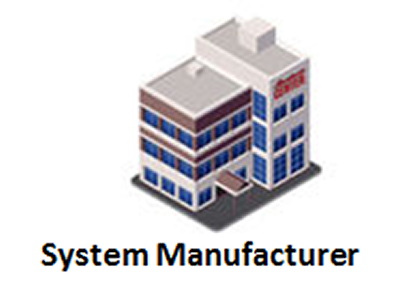
\includegraphics[width=\textwidth]{images/manufacturer}}
\end{minipage}

Before embarking on any hazard analysis, the manufacturer ensures that \index{Stakeholder}\glspl{stakeholder} review the general, historical perspective. This takes the form of a refresh briefing to raise awareness of issues that are specific to data such as ageing, biasing and defaults.

The manufacturer of the health IT System decides that during the prototyping phase there is little safety dependency of the test and \gls{configuration data} sets as no clinical decisions will be made based on their content; the data is simply being used to support the elaboration of requirements.

In later phases however, when the system functionality is specified and the system is being built, the manufacturer will want to create a test \gls{dataset} that will be instrumental in demonstrating the correct functioning of the system. This still involves the use of \gls{verification} data\index{Verification Data} and infrastructure data\index{Infrastructure Data}, but there is far greater dependency on these \glspl{dataset} than the previous case. For example, if the \gls{verification} or \gls{configuration data} is not sufficiently diverse or if it insufficiently models real-world scenarios, it is possible that erroneous and unsafe functional behaviour is present in the system during live operation despite the system having passed factory and site acceptance testing.

To analyse the risks in more detail, the manufacturer uses a top-down approach and a bottom-up approach. In the first approach it considers each of the system functions (such as clinical screens) and analyses where there is a dependency on data and what \index{Property!Data}properties need to be preserved. In the second, as much of the functionality is driven by data flows in and out of the system, the manufacturer also looks at specific data flows and assesses the impact of loss of \index{Property!Data}properties for the data in those flows.

On completion of the risk identification phase the manufacturer updates planning documents such as the clinical risk management plan, to reflect the outcome of the analysis.

\begin{minipage}[t]{0.73\textwidth}
  The health organization will likewise need to conduct risk identification relevant to their deployment context. \Glspl{hazard} arising from data sources that are to be delivered into the new system from existing systems need to be assessed for data risks.
  As with the manufacturer, a briefing to \index{Stakeholder}\glspl{stakeholder} to review the general, historical perspective is first conducted to cover generic data safety issues but also to highlight lessons learned from previous accidents and incidents that have occurred in the health organization itself.
\end{minipage}
\begin{minipage}[t]{0.25\textwidth}
  \centering\raisebox{\dimexpr \topskip-\height}{%
    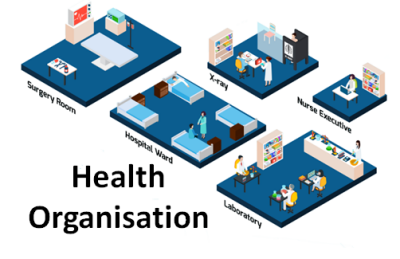
\includegraphics[width=\textwidth]{images/healthorganisation}}
\end{minipage}

As with the manufacturer, both a top-down approach and a bottom-up approach are adopted. From the health organization's perspective, one key focus for \gls{hazard} identification is in the use of dynamic data, i.e., data that will be delivered into the new system from existing system data sources and the data presented to the user. For the interactions identified in the supply chain, the health organization needs to consider the risks associated with loss of \index{Property!Data}properties of the data it will receive. Questions the health organization will need to consider and address more formally in the clinical risk management plan are:
\clearpage% Required on 3.3 to keep page breaks as 3.2
\begin{itemize}
  \item which \glspl{dataset} or \glspl{item data}\ being received from other systems have \index{Property!Data}\glspl{data property} (such as \gls{timeliness}\index{Timeliness Property}, \index{Completeness!Property}\gls{completeness}, \index{Consistency!Property}\gls{consistency}, \index{Fidelity / Representation Property}\gls{fidelity} etc.) that are significant to patient safety? 
  \item what data presented to the user has \index{Property!Data}\glspl{data property} (such as \index{Availability Property}\gls{availability}, format, \gls{resolution}\index{Resolution Property}, etc.) that are significant to patient safety?
  \item what existing barriers or \glspl{mitigation}\index{Mitigation} (physical, technical, procedural) exist to reduce the risk of loss of \index{Property!Data}\glspl{data property}? and
  \item will any existing barriers be lost as a consequence of the new system?
\end{itemize}

On completion of the Risk Identification phase the health organization will update planning documents such as the clinical risk management plan to reflect the outcome of the analysis.

\section{Risk Analysis}
\begin{minipage}[t]{0.73\textwidth}
  In this phase identified \glspl{hazard} are assessed to determine their likelihood and severity. To meet the guidance objectives the following activities are carried out:
  \begin{itemize}
    \item establish \glspl{dsal}\index{Assurance Level!Data}; and
    \item analyse \glspl{dsal} as part of system safety activities.
  \end{itemize}
\end{minipage}
\begin{minipage}[t]{0.25\textwidth}
  \centering\raisebox{\dimexpr \topskip-\height}{%
    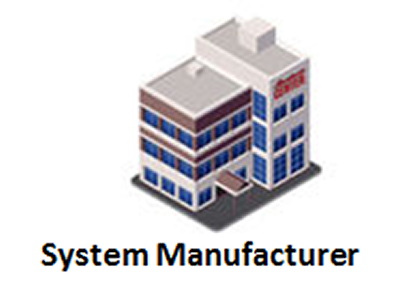
\includegraphics[width=\textwidth]{images/manufacturer}}
\end{minipage}

The manufacturer will establish \glspl{dsal}\index{Assurance Level!Data} by considering cases where the use of specific categories of data\index{Category!Data} could give rise to \glspl{hazard}. In the prototyping phase, the manufacturer sees no use of the data that can give rise to credible clinical risk and assesses the \gls{dsal}\index{Assurance Level!Data} for that \gls{dataset} as \dsiwgTextBF{DSAL0}. 

In the second phase of the development lifecycle\index{Lifecycle!Development}, where \gls{verification} data\index{Verification Data} and infrastructure data\index{Infrastructure Data} is being used to demonstrate the correct functioning of the system, the manufacturer considers that loss of any of the \glspl{data property} of \index{Integrity Property}\gls{integrity}, \index{Completeness!Property}\gls{completeness}, \index{Consistency!Property}\gls{consistency}, \index{Continuity Property}\gls{continuity}, \index{Format Property}\gls{format}, \index{Accuracy Property}\gls{accuracy}, \gls{resolution}\index{Resolution!Data}, \gls{timeliness}\index{Timeliness Property}, \index{Availability Property}\gls{availability}, \index{Fidelity / Representation Property}\gls{fidelity}, \gls{sequencing}\index{Sequencing, Data}, \gls{intended_destination}\index{Intended Destination / Usage Property}, \gls{goldilocks}\index{Goldilocks Property}, and explainability\index{Explainability Property} of this data could give rise to \glspl{hazard}.

For example, if the \gls{verification} \gls{dataset} selected is not representative of the eventual diversity experienced in practice (loss of \index{Fidelity / Representation Property}\gls{fidelity}), then it is possible that the system may contain latent software errors that could give rise to harm. However, the manufacturer acknowledges that the system will be subject to further testing and trials in the clinical setting and so there will be other opportunities to detect errors in the system. Overall:
\begin{itemize}
  \item the likelihood of the data use gives rise to an accident is \dsiwgTextBF{Medium} as other systems and processes are in place that would detect errors; and
  \item the severity is \dsiwgTextBF{Moderate}; failings in the system could give rise to non-optimal \index{Treatment!Medical}treatment plans for a patient that might delay detection of a more serious condition or prolong the recovery for a known condition.
\end{itemize}

The manufacturer therefore assesses these data categories\index{Category!Data} as \dsiwgTextBF{DSAL1}\index{Assurance Level!Data} in this particular context of use.

The manufacturer takes care to analyse \glspl{dsal}\index{Assurance Level!Data} as part of system safety activities by documenting these assessments along with other hardware and software safety considerations, for example those arising from DCB0129, in the clinical risk management plan.

\begin{minipage}[t]{0.73\textwidth}
  From the health organization's perspective, the main focus for risk assessment to establish \glspl{dsal}\index{Assurance Level!Data} is in the use of dynamic data\index{Dynamic Data}. For the interactions identified in the supply chain the health organization needs to consider the risks associated with loss of \index{Property!Data}properties of the data it will receive and present to the user. Questions the health organization will need to consider and address more formally in the clinical risk management plan are as follows:
\end{minipage}
\begin{minipage}[t]{0.25\textwidth}
  \centering\raisebox{\dimexpr \topskip-\height}{%
    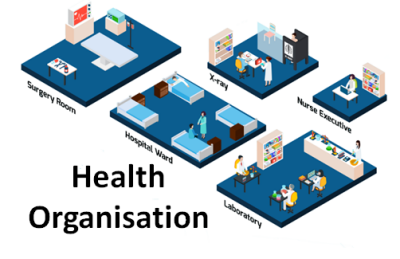
\includegraphics[width=\textwidth]{images/healthorganisation}}
\end{minipage}

\begin{itemize}
  \item how likely is it that there would be a loss of the given \index{Property!Data}\gls{data property}?
  \item how would such a loss of a \index{Property!Data}\glspl{data property} be detected?
  \item how would such as loss be isolated to prevent further risks of harm? and
  \item hhat recovery action would be required to resolve the issue to maintain patient safety?
\end{itemize}

Concerns were raised about the vulnerability of the system to inadvertent data overload from the large number of potential data sources, and possibly from malicious activity. This led to the addition of the \gls{goldilocks}\index{Goldilocks Property} property to the list of \index{Property!Data}\glspl{data property} applicable to the live system.

In considering the receipt of outcome measures data received from a clinic or hospital, the health organization considers that it is likely that some credible errors would not be readily detected by their new system; if the hospital system confused a result or there were errors in the precision of data then there would be few chances to catch these once received by the system.
\begin{itemize}
  \item The health organizations assesses the likelihood of this loss of \index{Property!Data}property as \dsiwgTextBF{High}; and
  \item The impact of such errors, although not realistically likely to lead to death, could result in delays to \index{Treatment!Medical}treatment that could result in serious injury and hence \dsiwgTextBF{Moderate} impact.
\end{itemize}

The data received from this data source is therefore classed as \dsiwgTextBF{DSAL2}\index{Assurance Level!Data} in this particular context of use.

The health organization takes care to analyse \glspl{dsal} as part of system safety activities by documenting these assessments along with other hardware and software safety considerations (e.g., arising from DCB0160 requirements) in the clinical risk management plan.

\section{Risk Evaluation and \index{Treatment!Risk}\Glsfmttext{treatment}}

\begin{minipage}[t]{0.73\textwidth}
  The manufacturer carries out the following activities to meet the guidance objectives:
  \begin{itemize}
    \item review each risk and either avoid, accept, transfer, \gls{treat};
    \item establish \index{Treatment!Risk} methods for relevant risks; and
    \item implement and verify \index{Treatment!Risk}\gls{treatment} methods.
  \end{itemize}
\end{minipage}
\begin{minipage}[t]{0.25\textwidth}
  \centering\raisebox{\dimexpr \topskip-\height}{%
    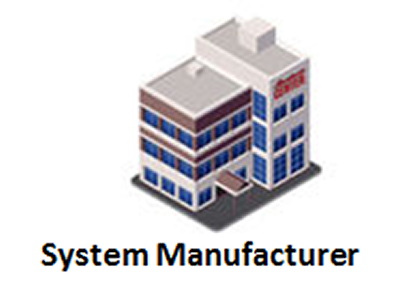
\includegraphics[width=\textwidth]{images/manufacturer}}
\end{minipage}

The manufacturer decides to review each risk and either avoid, accept, transfer, or \gls{treat} the risk. It decides to accept the \dsiwgTextBF{DSAL0}\index{Assurance Level!Data} risk, but as it has determined there is some, albeit low, risk (\dsiwgTextBF{DSAL1}) associated with its use of data at a specific point of its lifecycle\index{Lifecycle!Data}, it decides to \gls{treat} that risk. The manufacturer evaluates this risk and considers that the risks should be reduced further by taking some reasonably practicable steps.

Having decided that further risk reduction is necessary, the manufacturer needs to establish \index{Treatment!Risk}\gls{treatment} methods for relevant risks that are appropriate for DSAL1\index{Assurance Level!Data}data, and in doing so demonstrate that reasonably practicable steps have been taken to reduce the risk. The manufacturer therefore refers to the tables in the \gls{dsg} document. The manufacturer then documents in its clinical risk management plan:

\begin{itemize}
  \item planned compliance with the tables;
  \item the interpretation for the given method / technique (e.g.\ depth of checking); and
  \item justification in the case where a technique is not to be adopted.
\end{itemize}

For \dsiwgTextBF{DSAL1}\index{Assurance Level!Data} \gls{verification} data, the tables show that the following are recommended (R) or highly recommended (HR) where loss of \glspl{data property} 
	\gls{integrity}\index{Integrity Property},
	\gls{completeness}\index{Completeness!Property}, 
	\gls{consistency}\index{Consistency!Property},
	\gls{continuity}\index{Continuity Property},
	format\index{Format Property},
	\gls{accuracy}\index{Accuracy Property},
	\gls{resolution}\index{Resolution!Data},
	\gls{timeliness}\index{Timeliness Property},
	\gls{availability}\index{Availability Property},
	\gls{fidelity}\index{Fidelity / Representation Property},
	\gls{sequencing}\index{Sequencing, Data},
	\gls{intended_destination}\index{Intended Destination / Usage Property},
	\gls{goldilocks}\index{Goldilocks Property}, and
	\gls{explainability}\index{Explainability Property}
can give rise to
a number of \glspl{hazard}. The extracts below indicate the \gls{mitigation}\index{Mitigation} techniques identified from the tables which should form the basis of the \index{Safety Requirement!Data}\glspl{data safety requirement}. 

\begin{longtable}{|C{\dsiwgColumnWidth{0.08}}|L{\dsiwgColumnWidth{0.15}}|C{\dsiwgColumnWidth{0.08}}|L{\dsiwgColumnWidth{0.69}}|}
  \caption{Worked example: filtered techniques tables}
  \\\hline\TableHeadColourC{Ref} & \TableHeadColour{Technique} & \TableHeadColourCX{R / HR} & \TableHeadColour{System Design
  \hfill(extracted from \autoref*{tab:MethodsSystemDesign})
  }\\\hline
  \endfirsthead
  \caption[]{Worked example: filtered techniques tables (continued)}
  \\hline\TableHeadColourC{Ref} & \TableHeadColour{Technique} & \TableHeadColourCX{R/HR} & \TableHeadColour{System Design}\\\hline
  \endhead
  \multicolumn{4}{r}{\sl Continued on next page}
  \endfoot\endlastfoot
  SD.11 & Logging facilities & R & Data processing events are logged to allow support staff to monitor the health of the system and provide diagnostic \gls{information}.
  \\
  \hline
  SD.17 & Credibility / reasonability checks & R & Dedicated processing implemented to check that data is within reasonable tolerances and / or logically / semantically consistent (e.g., range checks, date checks, record counts, record sizes, special values - \gls{nan}). \\
  \hline
  SD.20 & Syntax checks & R & Semantic checking of data values and sequences based on defined rule sets.\\
  \hline
\end{longtable}

\addtocounter{table}{-1} % Kludge because longtable* is wrongly incrementing the table counter
\begin{longtable*}{|C{\dsiwgColumnWidth{0.08}}|L{\dsiwgColumnWidth{0.15}}|C{\dsiwgColumnWidth{0.08}}|L{\dsiwgColumnWidth{0.69}}|}
  \\\hline\TableHeadColourC{Ref} & \TableHeadColour{Technique} & \TableHeadColourC{R / HR} & \TableHeadColour{Data Design
  \hfill(extracted from \autoref*{tab:MethodsDataDesign})
  }\\\hline
  \endfirsthead
  \\\hline\TableHeadColourC{Ref} & \TableHeadColour{Technique} & \TableHeadColourC{R / HR} & \TableHeadColour{Data Design}\\\hline
  \endhead
  \endfoot\endlastfoot
  DD.01 & Governance model & R & A governance model is established that defines, e.g., \index{Data!Owner}data ownership, processing roles and responsibilities, processing authorizations and permissions.\\
  \hline
  DD.03 & Data flow diagram & HR & To describe the data flow in a diagrammatic form.\\
  \hline
  DD.04 & Data model & HR & To articulate how data is organized.\\
  \hline
  DD.05 & Client sign-off & R & Agreement from the client that the system architecture and design is appropriate for the data considered\\
  \hline
  DD.08 & Data dictionary & HR & A collection of descriptions of the data objects or \glspl{item data} in a data model for the benefit of data users.\\
  \hline
\end{longtable*}

\addtocounter{table}{-1} % Kludge because longtable* is wrongly incrementing the table counter
\begin{longtable*}{|C{\dsiwgColumnWidth{0.08}}|L{\dsiwgColumnWidth{0.15}}|C{\dsiwgColumnWidth{0.08}}|L{\dsiwgColumnWidth{0.69}}|}
  \\\hline\TableHeadColourC{Ref} & \TableHeadColour{Technique} & \TableHeadColourC{R / HR} & \TableHeadColour{Data Implementation
  \hfill(extracted from \autoref*{tab:MethodsDataProcedures})
  }\\\hline
  \endfirsthead
  \\\hline\TableHeadColourC{Ref} & \TableHeadColour{Technique} & \TableHeadColourC{R / HR} & \TableHeadColour{Data Implementation}\\\hline
  \endhead
  \endfoot\endlastfoot
   DI.01 & Review / inspection & HR & Manual review / inspection of data possibly involving data visualization tools.\\
  \hline
   DI.03 & Ground-truth check & R & Inspection against physical measurements (e.g., lengths, positions, heights) taken in the real world.\\
  \hline
   DI.04 & Auditing & R & A period of comprehensive internal and external testing of the data quality process.\\
  \hline
   DI.09 & Authorization & R & A security model is established to control who is authorized to create, view, edit, delete the data.\\
  \hline
   DI.11 & Defined confidence / Trust Levels & R & Criteria are established to provide an objective measurement of the confidence or trust in a given \gls{dataset}.\\
  \hline
\end{longtable*}

\addtocounter{table}{-1} % Kludge because longtable* is wrongly incrementing the table counter
\begin{longtable*}{|C{\dsiwgColumnWidth{0.08}}|L{\dsiwgColumnWidth{0.15}}|C{\dsiwgColumnWidth{0.08}}|L{\dsiwgColumnWidth{0.69}}|}
  \\\hline\TableHeadColourC{Ref} & \TableHeadColour{Technique} & \TableHeadColourC{R / HR} & \TableHeadColour{Data Migration
  \hfill(extracted from \autoref*{tab:MethodsDataMigration})
  }\\\hline
  \endfirsthead
  \\\hline\TableHeadColourC{Ref} & \TableHeadColour{Technique} & \TableHeadColourC{R / HR} & \TableHeadColour{Data Migration}\\\hline
  \endhead
  \endfoot\endlastfoot
  \multicolumn{4}{|l|}{No relevant techniques}\\
  \hline
\end{longtable*}

\addtocounter{table}{-1} % Kludge because longtable* is wrongly incrementing the table counter
\begin{longtable*}{|C{\dsiwgColumnWidth{0.08}}|L{\dsiwgColumnWidth{0.15}}|C{\dsiwgColumnWidth{0.08}}|L{\dsiwgColumnWidth{0.69}}|}
  \\\hline\TableHeadColourC{Ref} & \TableHeadColour{Technique} & \TableHeadColourC{R / HR} & \TableHeadColour{Data Checking
  \hfill(extracted from \autoref*{tab:MethodsDataChecking})
  }\\\hline
  \endfirsthead
  \\\hline\TableHeadColourC{Ref} & \TableHeadColour{Technique} & \TableHeadColourC{R / HR} & \TableHeadColour{Data Checking}\\\hline
  \endhead
  \endfoot\endlastfoot
  \multicolumn{4}{|l|}{No relevant techniques}\\
  \hline
\end{longtable*}

\addtocounter{table}{-1} % Kludge because longtable* is wrongly incrementing the table counter
\begin{longtable*}{|C{\dsiwgColumnWidth{0.08}}|L{\dsiwgColumnWidth{0.15}}|C{\dsiwgColumnWidth{0.08}}|L{\dsiwgColumnWidth{0.69}}|}
  \\\hline\TableHeadColourC{Ref} & \TableHeadColour{Technique} & \TableHeadColourC{R / HR} & \TableHeadColour{Test Data
  \hfill(extracted from \autoref*{tab:MethodsTestData})
  }\\\hline
  \endfirsthead
  \\\hline\TableHeadColourC{Ref} & \TableHeadColour{Technique} & \TableHeadColourC{R / HR} & \TableHeadColour{Test Data}\\\hline
  \endhead
  \endfoot\endlastfoot
   TD.01 & Using informal / ad-hoc means & R & Data is generated by simple means (e.g, spreadsheets, scripts, basic assumptions). There is no formal checking or review of the method of generation.\\
  \hline
   TD.05 & Using manual means & R & Simple test data can be produced by manual means, although this may be prone to human error.\\
  \hline
   TD.08 & Using initial runs of new system & R & This method is often used where the system is breaking new ground and there is no prototype or legacy system to produce test data. Initial operations may differ from eventual usage, so test data must evolve.\\
  \hline
   TD.09 & Derived from real data & R & Where real data is available this is usually a good basis for generating test data (e.g., by modification to increase the test space coverage).\\
  \hline
   TD.11 & Produced by client & R & Ideally the client is involved in producing or at least checking the test data.\\
  \hline
   TD.12 & Client sign-off & R & Where possible, the client should formally agree and sign off the test data as appropriate.\\
  \hline
   TD.13 & Error seeding & R & This is where errors are deliberately inserted into the \gls{dataset} to demonstrate the effectiveness of data \gls{validation}.\\
  \hline
   TD.14 & Data reuse & R & Reusing data for one project that was created and thoroughly assured for another project. This can be effective but the read-across should be established.\\
  \hline
   TD.15 & Feedback testing & R & To check output data by comparing it with the input source.\\
  \hline
\end{longtable*}

\addtocounter{table}{-1} % Kludge because longtable* is wrongly incrementing the table counter
\begin{longtable*}{|C{\dsiwgColumnWidth{0.08}}|L{\dsiwgColumnWidth{0.15}}|C{\dsiwgColumnWidth{0.08}}|L{\dsiwgColumnWidth{0.69}}|}
  \\\hline\TableHeadColourC{Ref} & \TableHeadColour{Technique} & \TableHeadColour{R / HR} & \TableHeadColour{Media -- paper
  \hfill(extracted from \autoref*{tab:MethodsDataMediaPhysical})
  }\\\hline
  \endfirsthead
  \\\hline\TableHeadColourC{Ref} & \TableHeadColour{Technique} & \TableHeadColour{R/HR} & \TableHeadColour{Media -- paper}\\\hline
  \endhead
  \endfoot\endlastfoot
  MP.01 & Photographic copies & R & Photocopy and store separately.\\
  \hline
  MP.02 & Scan to electronic format & R & Retain both paper and electronic copies.\\
  \hline
  MP.10 & Indexing / cataloguing & R & To support efficient availability.\\
  \hline
\end{longtable*}

\addtocounter{table}{-1} % Kludge because longtable* is wrongly incrementing the table counter
\begin{longtable*}{|C{\dsiwgColumnWidth{0.08}}|L{\dsiwgColumnWidth{0.15}}|C{\dsiwgColumnWidth{0.08}}|L{\dsiwgColumnWidth{0.69}}|}
  \\\hline\TableHeadColourC{Ref} & \TableHeadColour{Technique} & \TableHeadColourC{R / HR} & \TableHeadColour{Media -- electronic
  \hfill(extracted from \autoref*{tab:MethodsDataMediaElectronic})
  }\\\hline
  \endfirsthead
  \\\hline\TableHeadColourC{Ref} & \TableHeadColour{Technique} & \TableHeadColourC{R/HR} & \TableHeadColour{Media -- electronic}\\\hline
  \endhead
  \endfoot\endlastfoot
   ME.01 & Regular refresh / rewrite & R & Of magnetic media or flash memory.\\
  \hline
   ME.02 & Suitable physical environment & R & Store media in a clean, low-humidity environment at a steady temperature, cool but not cold.\\
  \hline
   ME.03 & Copies at different locations & R & Physically separate to cover natural disasters, accidental or malicious damage.\\
  \hline
   ME.04 & Backups / duplication & R & Backups are essential. Frequency of backup depends on rate of change. The number of generations to keep relates to the impact of data loss.\\
  \hline
   ME.05 & Sample restores & R & Sample restores should be performed at intervals to ensure that the backups are readable and retrievable.\\
  \hline
\end{longtable*}

From these tables the manufacturer decides on a series of activities to implement the recommendations that are applicable to its particular endeavour. These activities are expressed as a series of requirements that can be placed on the manufacturer's delivery organization and tracked through to completion. 

\begin{longtable}{|C{\dsiwgColumnWidth{0.07}}|L{\dsiwgColumnWidth{0.78}}|C{\dsiwgColumnWidth{0.15}}|}
\caption{Worked example: derived \glsentryplural{data safety requirement}\index{Safety Requirement!Data!Derived}}
  \\\hline\TableHeadColourC{} & \TableHeadColour{} & \TableHeadColourCX{Guidance}\\
  \multirow{-2}*{\TableHeadColourC{Ref}} & \multirow{-2}*{\TableHeadColour{Requirement}} & \TableHeadColourCX{Reference}\\\hline
  \endfirsthead
    \caption[]{Worked example: derived \glsentrylong{data safety requirement}\index{Safety Requirement!Data!Derived} (continued)}
  \\\hline\TableHeadColourC{} & \TableHeadColour{} & \TableHeadColourCX{Guidance}\\
  \multirow{-2}*{\TableHeadColourC{Ref}} & \multirow{-2}*{\TableHeadColour{Requirement}} & \TableHeadColourCX{Reference}\\\hline
  \endhead
      \multicolumn{3}{r}{\sl Continued on next page}
\endfoot\endlastfoot
  R1 & The \gls{verification} data shall be carefully controlled in the manufacturer's configuration management system. There shall be a configuration management plan that shall define who has responsibility for the data and who is authorized to create and amend it. & DD.01, DI.09\\
  \hline
  R2 & The \gls{verification} data shall be held on an industry standard file share that is regularly backed up with copies moved periodically to off-site storage. The Backup / Recovery plans shall include periodic sampling of restores. & ME.01, ME.02, ME.03, ME.04, ME.05\\
  \hline
  R3 & The data shall be modelled as a series of patient ``journeys'' that cover the entire lifecycle\index{Lifecycle!Data} of data from first encounter through to archival and deletion of data. The complete set of journeys shall be chosen to exercise all the functionality of the system. The modelling shall include a \gls{data dictionary}, data flow diagrams and a data model. & DD.03, DD.04, DD.08\\
  \hline
  R4 & To model data from external systems, the manufacturer shall use manual data entry\index{Data!Entry} and spreadsheet based records to hold the data. & TD.01, TD.05\\
  \hline
  R5 & The manufacturer has a set of clinical standing data that was used for another system and derived from real data.
  It includes encounter codes, clinical terms, consultant names, surgery and hospital addresses etc.\ and can be reused for this system. The manufacturer's Clinical Safety Officer has reviewed the data and agreed its suitability for reuse. & TD.09, TD.14\\
  \hline
  R6 & Some of the \gls{verification} \glspl{dataset} shall include errors deliberately inserted to check the effectiveness of data \gls{validation}. & TD.13\\
  \hline
  R7 & The controlled \gls{verification} \gls{dataset} shall be subject to review and analysis against defined confidence / trust criteria. Scripts shall be written to check for syntax and semantic \index{Consistency!Semantic}\gls{consistency} of the data and provide a basic  credibility check. The scripts themselves shall be validated and verified before use. & SD.17, SD.20, DI.01, DI.03, DI.11\\
  \hline
  R8 & The project shall be subject to an internal delivery quality assurance audit. & DI.04\\
  \hline
  R9 & Data loaded from external system into the system and displayed to the user shall be crosschecked against the original source data, using manual spot-checks. & TD.15\\
  \hline
  R10 & The level of rigour employed in verifying all the above requirements shall be commensurate with the \gls{dsal}\index{Assurance Level!Data} \gls{criticality} and so an ISO9001 compliant quality management system shall be adopted. & All\\
  \hline
  R11 & Data processing events shall be logged to allow monitoring of the health of the system, provide diagnostic \gls{information}, allow audit trails and support the production of explanations. & SD.11\\
  \hline
  R12 & Each contracted client will be asked to ensure and signoff that test, configuration and adaptation data is appropriate (eg. in terms coverage and representative of real-life values) for their particular circumstance. & DD.05, TD.11, TD.12\\
  \hline
\end{longtable}

The following guidance recommendations were not adopted by the manufacturer for the reasons given. Note that some may however become relevant in the future so actions are set, where appropriate, to review the applicability of the recommendation when the given condition is met.

\begin{longtable}{|C{\dsiwgColumnWidth{0.07}}|C{\dsiwgColumnWidth{0.13}}|L{\dsiwgColumnWidth{0.55}}|L{\dsiwgColumnWidth{0.25}}|}
\caption{Worked example: \index{Safety Requirement!Data!Rejected}rejected data safety requirements}
  \\\hline\TableHeadColourC{} & \TableHeadColourC{Guidance} & \TableHeadColour{} & \TableHeadColourCX{}\\
  \multirow{-2}*{\TableHeadColourC{Ref}} & \TableHeadColourC{Reference} & \multirow{-2}*{\TableHeadColour{Justification}} & \multirow{-2}*{\TableHeadColourCX{Action}}\\\hline
  \endfirsthead
\caption[]{Worked example: \index{Safety Requirement!Data!Rejected}rejected \glsentryplural{data safety requirement} (continued)}
  \\\hline\TableHeadColourC{} & \TableHeadColourC{Guidance} & \TableHeadColour{} & \TableHeadColourCX{}\\
  \multirow{-2}*{\TableHeadColourC{Ref}} & \TableHeadColourC{Reference} & \multirow{-2}*{\TableHeadColour{Justification}} & \multirow{-2}*{\TableHeadColourCX{Action}}\\\hline
  \endhead
      \multicolumn{4}{r}{\sl Continued on next page}
  \endfoot\endlastfoot
  E1 & TD.08 & The data will be used before any initial run of the system. & Review when data from initial runs is available.\\
  \hline
  E2 & MP.01, MP.02, MP.10 & There are no paper based resources for this system. & No further action.\\
  \hline
\end{longtable}

Having determined the requirements arising from the data safety analysis the manufacturer ensures these are included along with other system requirements as part of the overall delivery and operation of the system. It then remains for the manufacturer to implement and verify \index{Treatment!Risk} methods, that is, as well as defining requirements the clinical risk management plan needs to ensure activities are in place to verify and evidence that \index{Treatment!Risk}\glspl{treatment} have actually been implemented.

\begin{minipage}[t]{0.79\textwidth}
  Likewise, the health organization has identified DSAL2\index{Assurance Level!Data} data and in deciding to \gls{treat} the risk, it aims to ensure risks are reduced as low as reasonably practicable. 
\end{minipage}
\begin{minipage}[t]{0.2\textwidth}
  \centering\raisebox{\dimexpr \topskip-\height}{%
    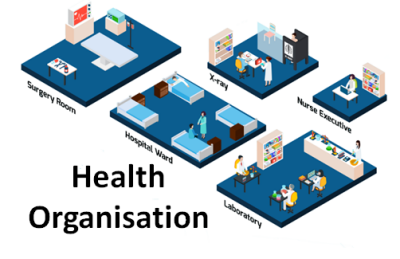
\includegraphics[width=\textwidth]{images/healthorganisation}}
\end{minipage}

